\title{Matrix Addition and Scalar Multiplication}
\subtitle{\SubTitleName}
\institute[]{\Course}
\author{\Instructor}
\maketitle   


\tikzstyle{startstop} =[trapezium, trapezium left angle=70, trapezium right angle=110, minimum width=1cm, minimum height=1cm, text centered, fill=Teal!30]

\tikzstyle{io} = [trapezium, trapezium left angle=70, trapezium right angle=110, minimum width=1cm, minimum height=1cm, text centered, fill=DarkRed!30]

\tikzstyle{process} = [trapezium, trapezium left angle=70, trapezium right angle=110, minimum width=1cm, minimum height=1cm, text centered, fill=Gold!60]

\tikzstyle{arrow} = [thick,->,>=stealth]

\frame{\frametitle{Topics and Objectives}
    \Emph{Topics} \\
    \TopicStatement
    \begin{itemize}
    
        \item identity and zero matrices
        
        \item matrix algebra: sums and scalar multiplies
        
    \end{itemize}
    
    \vspace{0.5cm}
    
    \Emph{Objectives}\\
    
    \LearningObjectiveStatement
    
    \begin{itemize}
    
        \item apply matrix algebra and the zero and identity matrices to solve and analyze matrix equations

    \end{itemize}


}



\frame{\frametitle{Definitions: Zero and Identity Matrices}

    \begin{itemize}

    \item A \Emph{zero matrix} is any matrix whose every entry is zero. 
    
    \begin{equation*}
        0_{2 \times 3} = 
        \begin{pmatrix}
            0 & 0 & 0\\ 0 & 0 & 0
        \end{pmatrix}
        , \quad 
        0_{2 \times 1} = 
        \begin{pmatrix}
            0 \\ 0
        \end{pmatrix}
    \end{equation*}    
    
    \pause 
    
    \item  The $n\times n$ \Emph{identity matrix} has ones on the main diagonal, otherwise all zeros. 
    \begin{equation*}
        I _{2} = 
        \begin{pmatrix}
            1 & 0 \\ 0 & 1 
        \end{pmatrix}
        , \quad 
        I _{3} = 
        \begin{pmatrix}
            1 & 0 & 0 \\ 0 & 1 & 0 \\ 0 & 0 & 1 
        \end{pmatrix}
    \end{equation*}
    
    \end{itemize}
    
    \pause 

    Note: any matrix with dimensions $n\times n$ is \Emph{square}. Zero matrices need not be square, identity matrices must be square. 

}

\begin{frame}
\frametitle{Matrix Addition and Scalar Multiples}

Suppose $ A$ and $B $ are $ m \times n$ matrices. \pause $a _{i,j}$ is the entry of $A$ in row $i$ and column $j$, and \pause $b _{i,j}$ is the entry of $B$ in row $i$ and column $j$. 

\begin{itemize}

    \item The entries of $ A+B$ are $a_{i,j} + b_{i,j}$. 

    \item If $ c \in \mathbb R$, then the entries of $c A$ are $c a _{i,j}$.  

\end{itemize}
\pause 
For example, if 

$$
\begin{pmatrix} 1 & 2 & 3 \\ 4 & 5 & 6 \end{pmatrix} + c
\begin{pmatrix} 7 & 4 & 7 \\ 0 & 0 & k \end{pmatrix} =
\begin{pmatrix} 15 & 10 & 17 \\ 4 & 5 & 16 \end{pmatrix}
$$
What are the values of $c$ and $k$?

\end{frame}





\frame{\frametitle{Properties of Sums and Scalar Multiples}

Scalar multiples and matrix addition have the expected properties. \\[12pt] If $ r, s \in \mathbb R $ are scalars, and $ A, B, C$ are $ m \times n$ matrices, then 
%%  ENUMERATE
\begin{enumerate}
\item<1->  $ A + 0 _{m \times n} = A$
\item<2->  $ (A+B) + C = A + (B+C)$
\item<3-> $ r (A+B) = r A + r B $ 
\item<4-> $ (r+s) A = r A + s A $ 
\item<5->  $ r (sA) = (rs) A$ 
\end{enumerate}
%% ENUMERATE

}


\frame{\frametitle{Summary}

    \SummaryLine \vspace{4pt}
    \begin{itemize}\setlength{\itemsep}{8pt}
        \item the identity and zero matrices
        \item matrix algebra: sums and scalar multiplies
    \end{itemize}
    \vspace{4pt}
    % There are several ways of multiplying matrices that we explore in this class. This video introduced two methods. 
}




% \frame{\frametitle{Matrix Multiplication}


% \begin{center}\begin{tikzpicture} \node [mybox](box){\begin{minipage}{0.80\textwidth}

% Let $ A $ be a $ m \times n $ matrix, and $ B$ be a $ n \times p$ matrix. The product is  $ A B  $ a $ m \times p$ matrix, equal to $$ A B = A 
% \begin{pmatrix}
% \vec b_1 & \cdots & \vec b_p
% \end{pmatrix} = 
% \begin{pmatrix}
% A \vec b_1 & \cdots & A \vec b_p
% \end{pmatrix}
% $$ 
% \end{minipage}};
% \node[fancytitle, right=10pt] at (box.north west) {Definition};
% \end{tikzpicture}\end{center}

%     \Emph{Example} \\
    
%     Compute the following product. 
    
%     \begin{equation*}
%     C = AB = 
%     \spalignmat{2 0;1 1}\spalignmat{2 0 0;3 4 0}
%     \end{equation*}

% }


% \frame{\frametitle{Row Column Rule for Matrix Multiplication }

%     The Row Column Rule is a convenient way to calculate the product $AB$ that many students have encountered in pre-requisite courses. 
    
%     \begin{center}\begin{tikzpicture} \node [mybox](box){\begin{minipage}{0.80\textwidth}
    
%     If $A \in \mathbb R^{m\times n}$ has rows $\vec a_i$, and $B \in \mathbb R^{n \times p}$ has columns $\vec b_j$, each element of the product $C=AB$ is the dot product $c_{ij} = \vec a_i \cdot \vec b_j$.
%     \end{minipage}};
%     \node[fancytitle, right=10pt] at (box.north west) {Row Column Method};
%     \end{tikzpicture}\end{center}
    
%     \Emph{Example} \\
    
%     Compute the following using the row-column method. 
    
%     \begin{equation*}
%     C = AB = 
%     \spalignmat{2 0;1 1}\spalignmat{2 0 0;3 4 0}
%     \end{equation*}


% }

% \frame{\frametitle{Matrix Dimensions and Matrix Multiplication}

%     Note: the dimensions of $A$ and $B$ determine whether $AB$ is defined, and what its dimensions will be.
    
%     \begin{center}
%         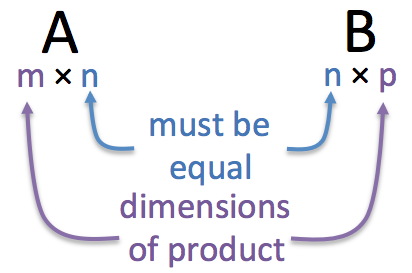
\includegraphics[width=0.3\textwidth]{Chapter2/images/matrix_multi2} 
%     \end{center}

% }



% \frame{\frametitle{Properties of Matrix Multiplication} 

%     Let $ A, B, C$ be matrices of the sizes needed for the matrix multiplication to be defined, and $ A $ is a $ m \times n$ matrix. 
    
%     \begin{enumerate}
%         \item (Associative)  $(AB)C= A (BC)$ 
%         \item (Left Distributive)  $A (B+C) = AB + AC $ 
%         \item (Right Distributive) $(A + B)C = AC + AC $ 
%         \item (Identity for matrix multiplication)  $ I _{m} A = A I _{n}$ 
%     \end{enumerate}

    
%     \Emph{\color{Teal}Warnings:}  
%     \begin{enumerate}
%         \item  (non-commutative)    In general, $ AB \neq BA $.   
%         \item  (non-cancellation)  $ AB = A C $ does not mean $ B=C$. 
%         \item  (Zero divisors)   $ AB = 0$ does not mean that either $ A=0$ or $ B=0$.  
%     \end{enumerate}

% }

% \frame{\frametitle{Examples}
%     Suppose $A = \spalignmat{1 0; 0 0}$.
%     \begin{enumerate}
%         \item Give an example of a $2\times2$ matrix that does not commute with $A$. 
%         \item Construct any non-zero matrices $B$ and $C$ so that $B\ne C$ but $AB=BC$.
%     \end{enumerate}
    
% }


% \frame{\frametitle{The Associative Property} 

%     If $C = \vec x$, then the associative property is: $(AB)\vec x = A (B \vec x)$. Schematically: 
    
%     \vspace{18pt}
    
%     \begin{tikzpicture}[node distance=2cm]

%         \node(x)  [startstop] {$\vec x$};
%         \node(bx) [io, below of=x] {$B\vec x$};
%         \node(abx)[process, right of=x,xshift=4cm]{$AB\vec x$};
        
%         \draw [arrow] (x) -- node[anchor=east] {\small Multiplication by $B$} (bx);
%         \draw [arrow] (bx) -- node[anchor=north,xshift=1.2cm] {\small Multiplication by $A$} (abx);
%         \draw [arrow] (x) --node[anchor=south] {\small  \ \ \ Multiplication by $AB$} (abx);
        
%     \end{tikzpicture}

%     \vspace{4pt}

%     The matrix product $ AB\vec x$ can be obtained by either: multiplying by matrix $AB$, or by multiplying by $B$ then by $A$. This means that matrix multiplication corresponds to \Emph{composition of the linear transformations}.
% }

% % 


% % \begin{frame}
% % \frametitle{Additional Examples}

% %     True or false:

% %     \begin{enumerate}
% %         \item For any $I_n$ and any $A \in \R^{n\times n}$, $(I_n + A)(I_n - A) = I_n - A^2$. \\[3cm]
% %         \item For any $A$ and $B$ in $\R^{n\times n}$, $(A+B)^2 = A^2 + B^2 + 2AB$. 
% %     \end{enumerate}

% % \end{frame}

% \frame{\frametitle{Summary}

%     \SummaryLine \vspace{4pt}
%     \begin{itemize}\setlength{\itemsep}{8pt}
%         \item the identity and zero matrices
%         \item matrix algebra: sums and products, scalar multiplies
%     \end{itemize}
%     \vspace{4pt}
%     There are several ways of multiplying matrices that we explore in this class. This video introduced two methods. 
% }
